\documentclass[diplomskirad]{fer}

\usepackage{booktabs}
\usepackage{listings}
\usepackage[outputdir=out]{minted}

\title{Dynamic fluid visualization using smoothed particle hydrodynamics method}
\naslov{Vizualizacija dinamike fluida metodom hidrodinamike zaglađujućih čestica}
\brojrada{542}
\mentor{Krešimir Trontl}
\author{Hrvoje Hemen}
\date{June, 2024}
\datum{lipanj, 2024.}
\begin{document}
    \maketitle
    \zadatak{HrvojeHemenZadatak.pdf}
    \begin{zahvale}
        Želim se zahvaliti mentoru Krešimiru Trontlu-
    \end{zahvale}
    \mainmatter
    \tableofcontents
% TEKST RADA
    \chapter{Uvod}\label{ch:uvod}

    \section{Cilj rada}\label{sec:cilj-rada}

    Cilj ovog rada bio je napraviti realnu simulaciju dinamike fluida.
    Korištena metoda bila je metoda hidrodinamike zaglađujućih čestica (SPH).
    Inspiracija za ovaj rad bio je jedan YouTube video Sebastiana Laguea koji govori o simulaciji vode u Unityju.

    \section{Ukratko o radu}\label{sec:ukratko-o-radu}

    U sklopu ovog rada obrađeno je sve potrebno za samostalnu izradu ovog rada uključujući i postavljanje razvojnog okruženja.

    Rad je pisan u c\# programskom jeziku u sklopu Unityja, te je za vizualizaciju korišten Unityjev dvodimenzionalni vizualizator.


    \chapter{Tehnologije}\label{ch:tehnologije}

    \section{C\#}\label{sec:c}

    \begin{figure}[H]
        \centering
        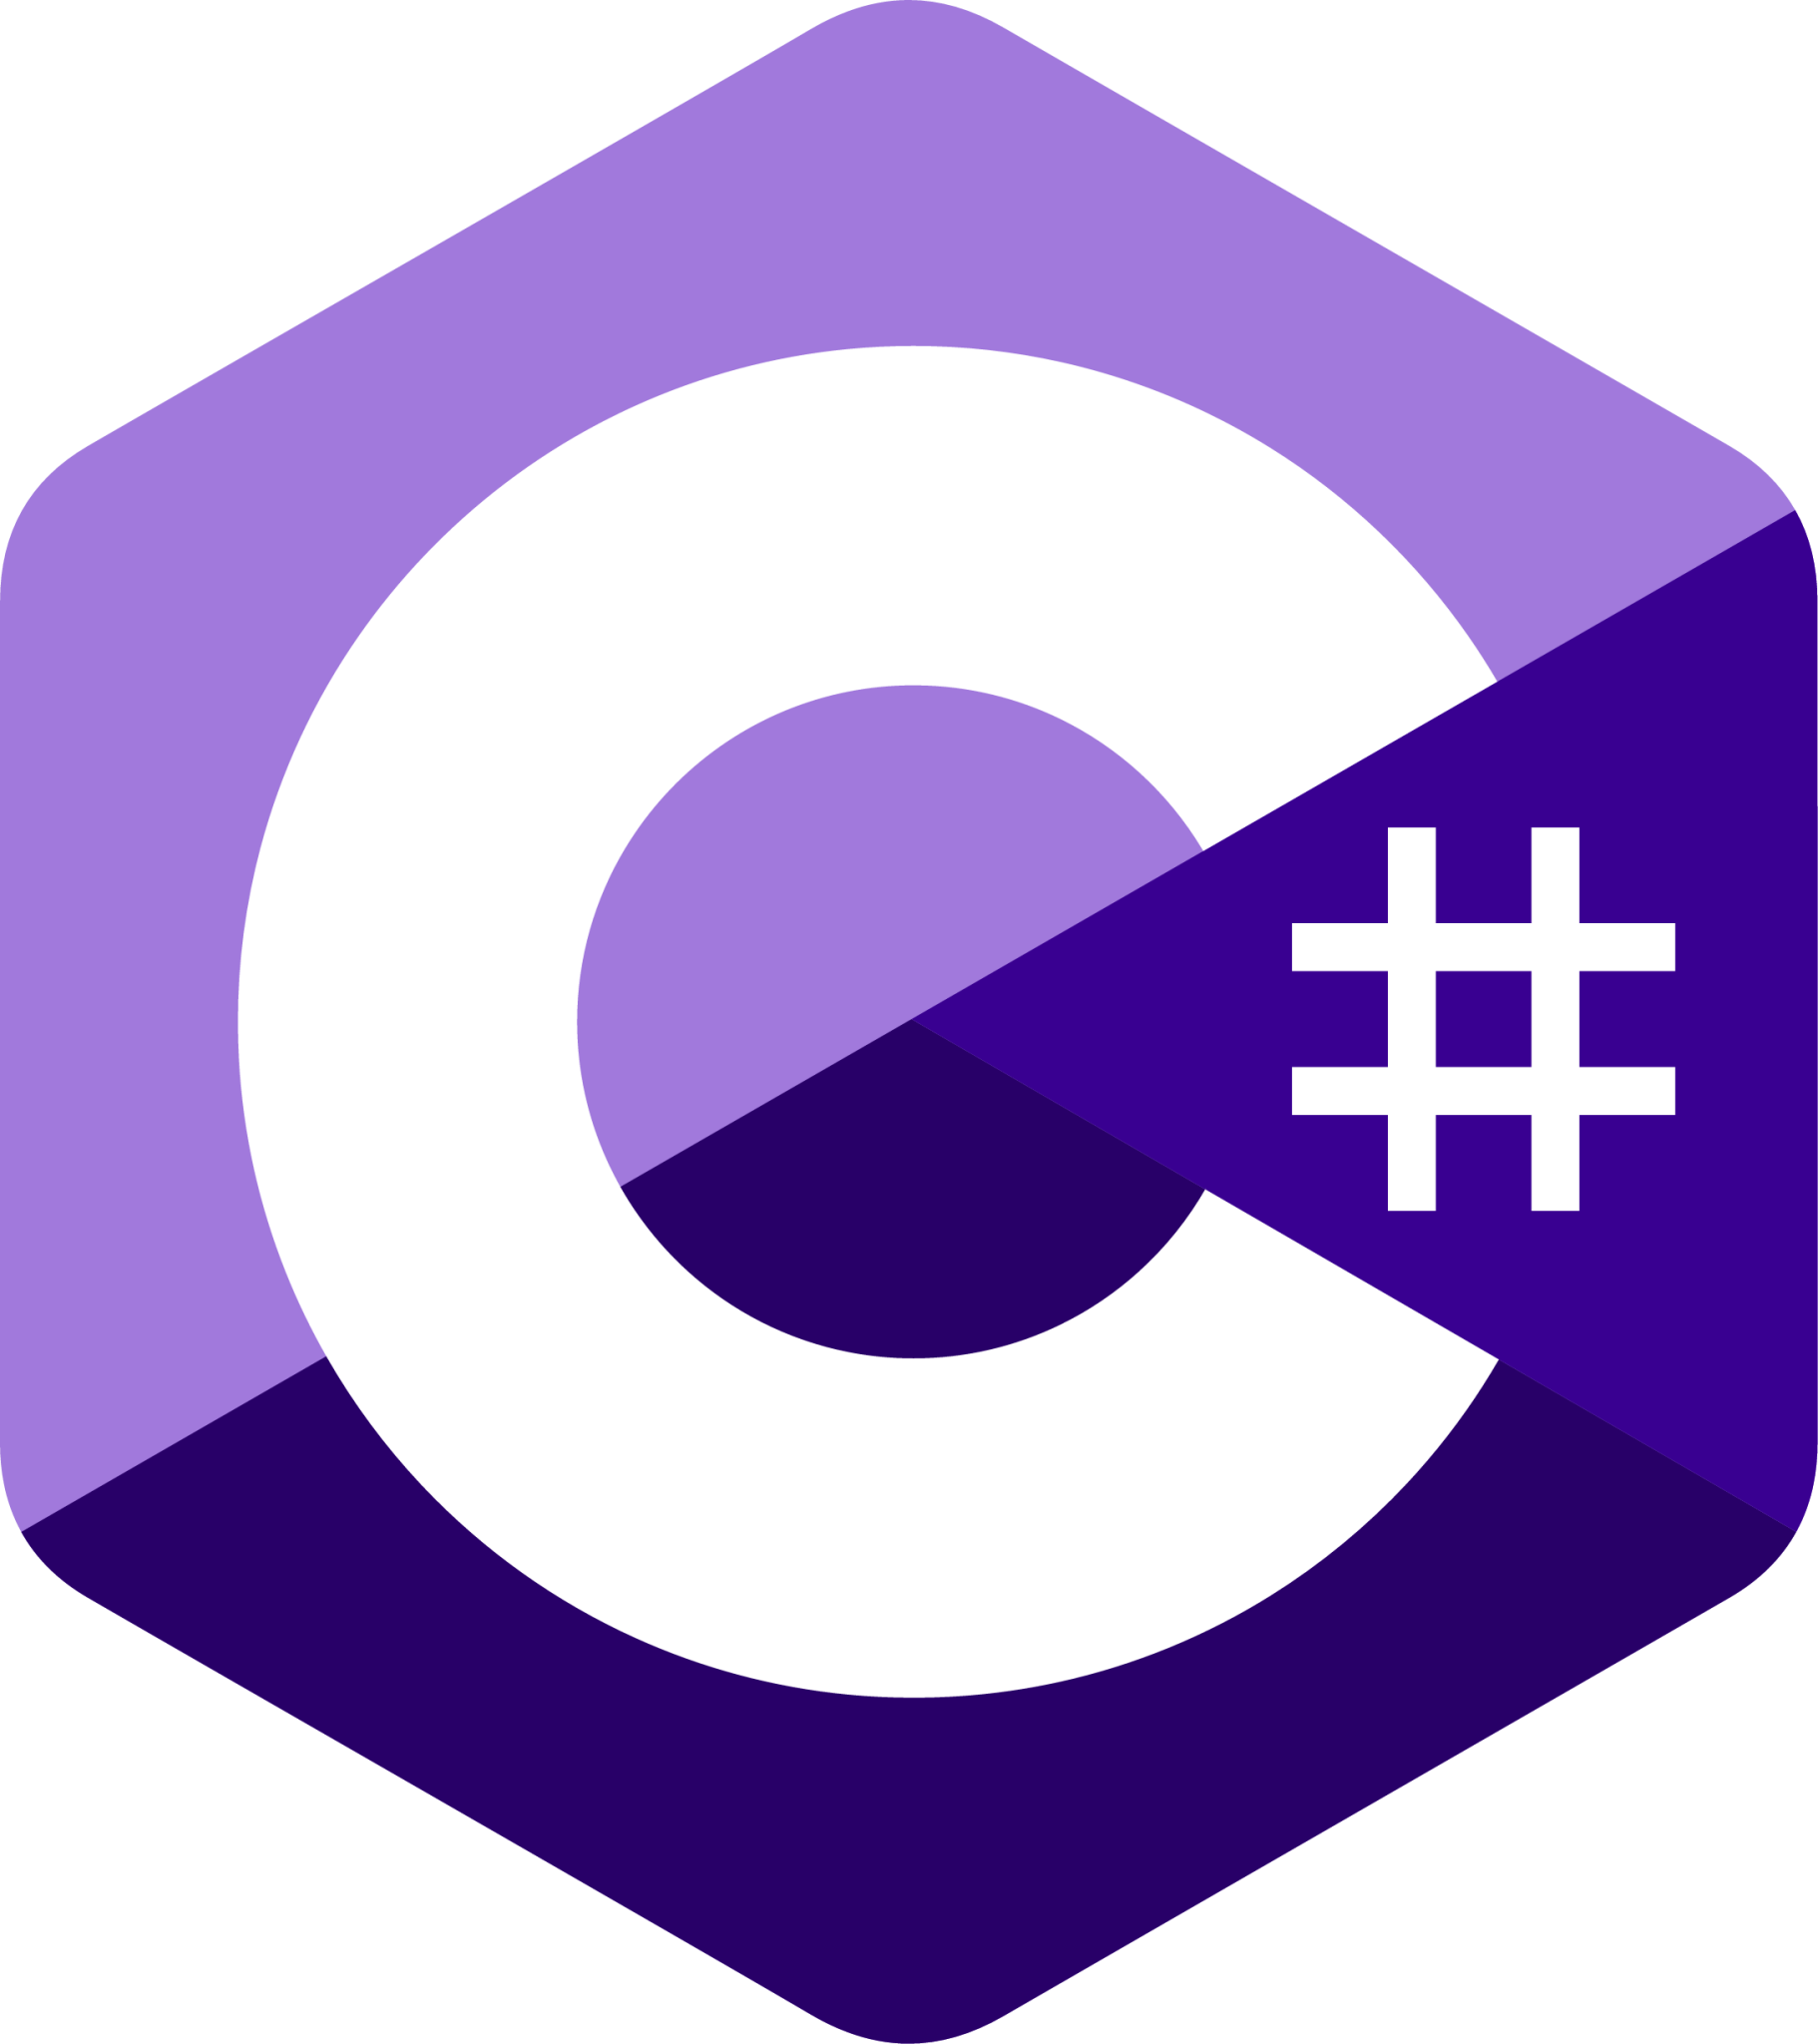
\includegraphics[scale=0.1]{images/c-sharp}
        \caption{
            C Sharp Logo \cite{cSharpLogo}
        }
        \label{fig:cSharpLogo}
    \end{figure}

    C\# je objektno orijentirani programski jezik visoke razine.
    Nastao je ranih 2000-ih zbog potrebe za objektno orijentiranim jezikom sintakse slične C jeziku.
    Najvažni ciljevi njegovog razvoja bili su jednostavnost, stroga tipiziranost,
    laka prijenosnost na različite operacijske sustave i mala potrošnja računalnih resursa.

    Sintaksa je vrlo slična Javinoj, jer svaka naredba treba završiti sa točka-zarezom \";\".
    Također, dijelovi koda omeđeni su vitičastim zagradama, koje razdvajaju kod u Klase i Metode.
    Važna razlika C\# i Jave je to što C\# omogućava preopterećenje osnovnih operacija, dakle možemo reći klasi da kada
    upotrijebimo znak plus onda radi nešto drugo, a ne matematičko dodavanje.


    \newpage
    \section{Unity}\label{sec:unity}

    \begin{figure}[H]
        \centering
        
\includegraphics[scale=0.3]{images/unityLogo}
        \caption{
            Unity Logo \cite{unityLogo}
        }
        \label{fig:unityLogo}
    \end{figure}

    Unity je razvojno okruženje i pogonski sklop za igre s mogućnosti razvoja 2D, 2.5D i 3D igara.
    Unity je nastao 2005 godine i od tada se kontinuirano raste i zauzima sve veći dio tržišta.

    Velika prednost Unityja nad drugim sličnim produktima je pristupačnost i opsežna dokumentacija.
    Pošto Unity omogućava razvoj za mobitele, Desktop platforme, web platforme, konzole te platforme virtualne realnosti,
    vrlo je jednostavno istu igru napraviti za više platformi.

    Postoji više licenci, među kojima postoji i besplatna razina.
    Ona omogućava novim programerima igara ulazak u taj svijet, te oni besplatno mogu vidjeti je li to za njih.



    \chapter{Teorijska podloga}\label{ch:teorijska-podloga}

    \section{Pristupi računalnoj simulaciji fluida}\label{sec:pristupi-racunalnoj-simulaciji-fluida}

    Kada pričamo o simulaciji fluida, najčešće mislimo na SPH metodu koju ovaj rad obrađuje, no postoji još mnogo
    različitih pristupa simulaciji fluida.
    Većina ih koristi čestice te simulira fluid nad njima, no neke koriste polja te pomoću njega računaju vizualiziraju čestice.

    \subsection{Simulacije bazirane na česticama}\label{subsec:simulacije-bazirane-na-cesticama}

    Simulacije bazirane na česticama su najintuitivnije.
    Svaka čestica predstavlja jednu česticu vode, te sadrži njena svojstva poput mase, brzine i vektora smjera kretanja.
    Kasnije se izračunavaju među-čestične sile poput tlaka i gustoće te se pomoću njih određuju nova svojstva čestica u
    sljedećem koraku simulacije te se to ponavlja.

    Najpoznatije simulacije ovog tipa su SPH koje će biti obrađeno zasebno, te DEM - Metoda diskretnih elemenata.

    DEM\cite{DEMmethod} metoda je većinski korištena za simulaciju građevinskog materijala poput piljevine ili pijeska.
    Ona uzima u obzir međučestične sile poput trenja, elastičnosti, i stavlja velik naglasak na Newtonove zakone.
    Najčešće se koristi u rudarskom inžinjerstvu, no postoje i primjene u farmaceutskoj industriji.

    \newpage
    \subsection{Simulacije bazirane na 2D polju}\label{subsec:simulacije-bazirane-na-2d-polju}

    Simulacije bazirane na 2D polju ne koriste čestice kao prijašnje metode, nego koriste 2D polje, u koje spremaju
    svojstva čestica koje bi se nalazile u ćeliji tog polja.
    One se kao i ostale simulacije izvode korak po korak.
    Ako želimo veliku simulaciju, njena složenost raste kvadratno, pa ove simulacije nisu prigodne za velike površine,
    baš zbog te velike računske složenosti.

    \begin{figure}[H]
        \centering
        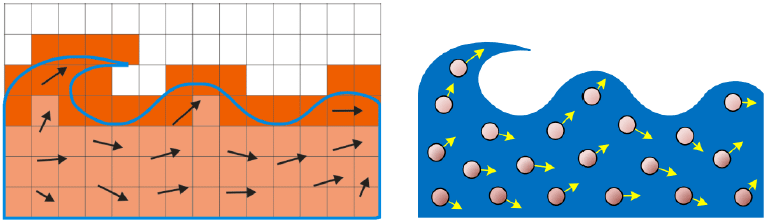
\includegraphics[scale=0.5]{images/gridBasedParticleBased}
        \caption{
            Grid based, Particle based simulation \cite{gridBasedParticleBased}
        }
        \label{fig:gridBasedParticleBased}
    \end{figure}

    \section{SPH metoda}\label{sec:sph-metoda}

    \subsection{Općenito o metodi}\label{subsec:opcenito-o-metodi}

    SPH metoda je računska metoda koja se koristi za simulaciju fluida.
    Ona je simulacija bazirana na česticama, te njihova svojstva koristi za računanje istih iz koraka u korak.
    Ona ne zahtjeva 2D polje, što je velika prednost, jer može simulirati fluid u složenim i nepravilnim prostorima.
    Njena složenost gledana s obzirom na broj čestica je puno manja nego složenost simulacija koje koriste 2D polje kada je gustoća jednaka.


    \chapter{Programska implementacija}\label{ch:programska-implementacija}

    \section{Osnove Unity okruženja}\label{sec:osnove-unity-okruzenja}
    \section{Osnove Unity fizičkog simulatora}\label{sec:osnove-unity-fizickog-simulatora}
    \section{Čestica}\label{sec:cestica}
    \section{Gustoća}\label{sec:gustoca}
    \section{Pritisak}\label{sec:pritisak}
    \section{Viskoza}\label{sec:viskoza}
    \section{Rezultantna sila}\label{sec:rezultantna-sila}


    \bibliography{literatura}
    \begin{sazetak}
        sažetak na hrvatskom
    \end{sazetak}
    \begin{kljucnerijeci}
        ključne riječi na hrvatskom
    \end{kljucnerijeci}
    \begin{abstract}
        abstract in English
    \end{abstract}
    \begin{keywords}
        keywords in English
    \end{keywords}
\end{document}